\subsection{State\_Fsm \& Display}

Once the password has been entered, it is displayed in the 4 7-segment displays. This display must show the entered four digit password and the “Open” or “Error” messages, depending on whether code is correct or not. Since all of the checking/validating code cannot fit in one GAL. the display must be able to be controlled by different GAL devices.\medskip

In order to display the entered password, two different GALs, State\_FSM and Display, will be used due to the length of the code. We will go over the "Open"/"Error" messages later.\medskip


{\subsubsection{State\_Fsm} }
\medskip

STATE\_FSM has as input the clock (\textit{CLK}), the \textit{RESET} signal, the output FSM states from the SAFECODE (\textit{S}) as inputs as well (As we discussed in \textbf{Subsubsection \ref{sec:WRITING_OPERATION}}), and the \textit{DONE} signal as output. \medskip

Most of the GALs of this project use FSMs to command the different operations, including this one. We will now go over the different states that form the State Machine:

\medskip
    \bm{$Q_0$}
\medskip

Initially, \textit{DONE}  is in a LOW level, then, the Final State Machine begins. The first state, \textit{$Q_0$}, pulls \textit{DONE} LOW, and changes to the next state if the read state from the safecode \textit{S} $= 00$. 

\medskip
{\textbf{\textit{\bm{$Q_1$}, \bm{$Q_2$} and return to \bm{$Q_0$}}}}
\medskip

At \textit{$Q_1$}, DONE remains the same, and once \textit{S} $= 10$, that is, the second state of the SAFECODE, DONE is pulled HIGH and the state changes to \textit{$Q_2$}. No changes occur in \textit{$Q_2$} until RESET is in HIGH level, then the state becomes \textit{$Q_0$}, effectively resetting the GAL.

\clearpage

To illustrate the different states and the transitions between them we have included the following diagram:\medskip

\begin{figure}[H]
    \centering
    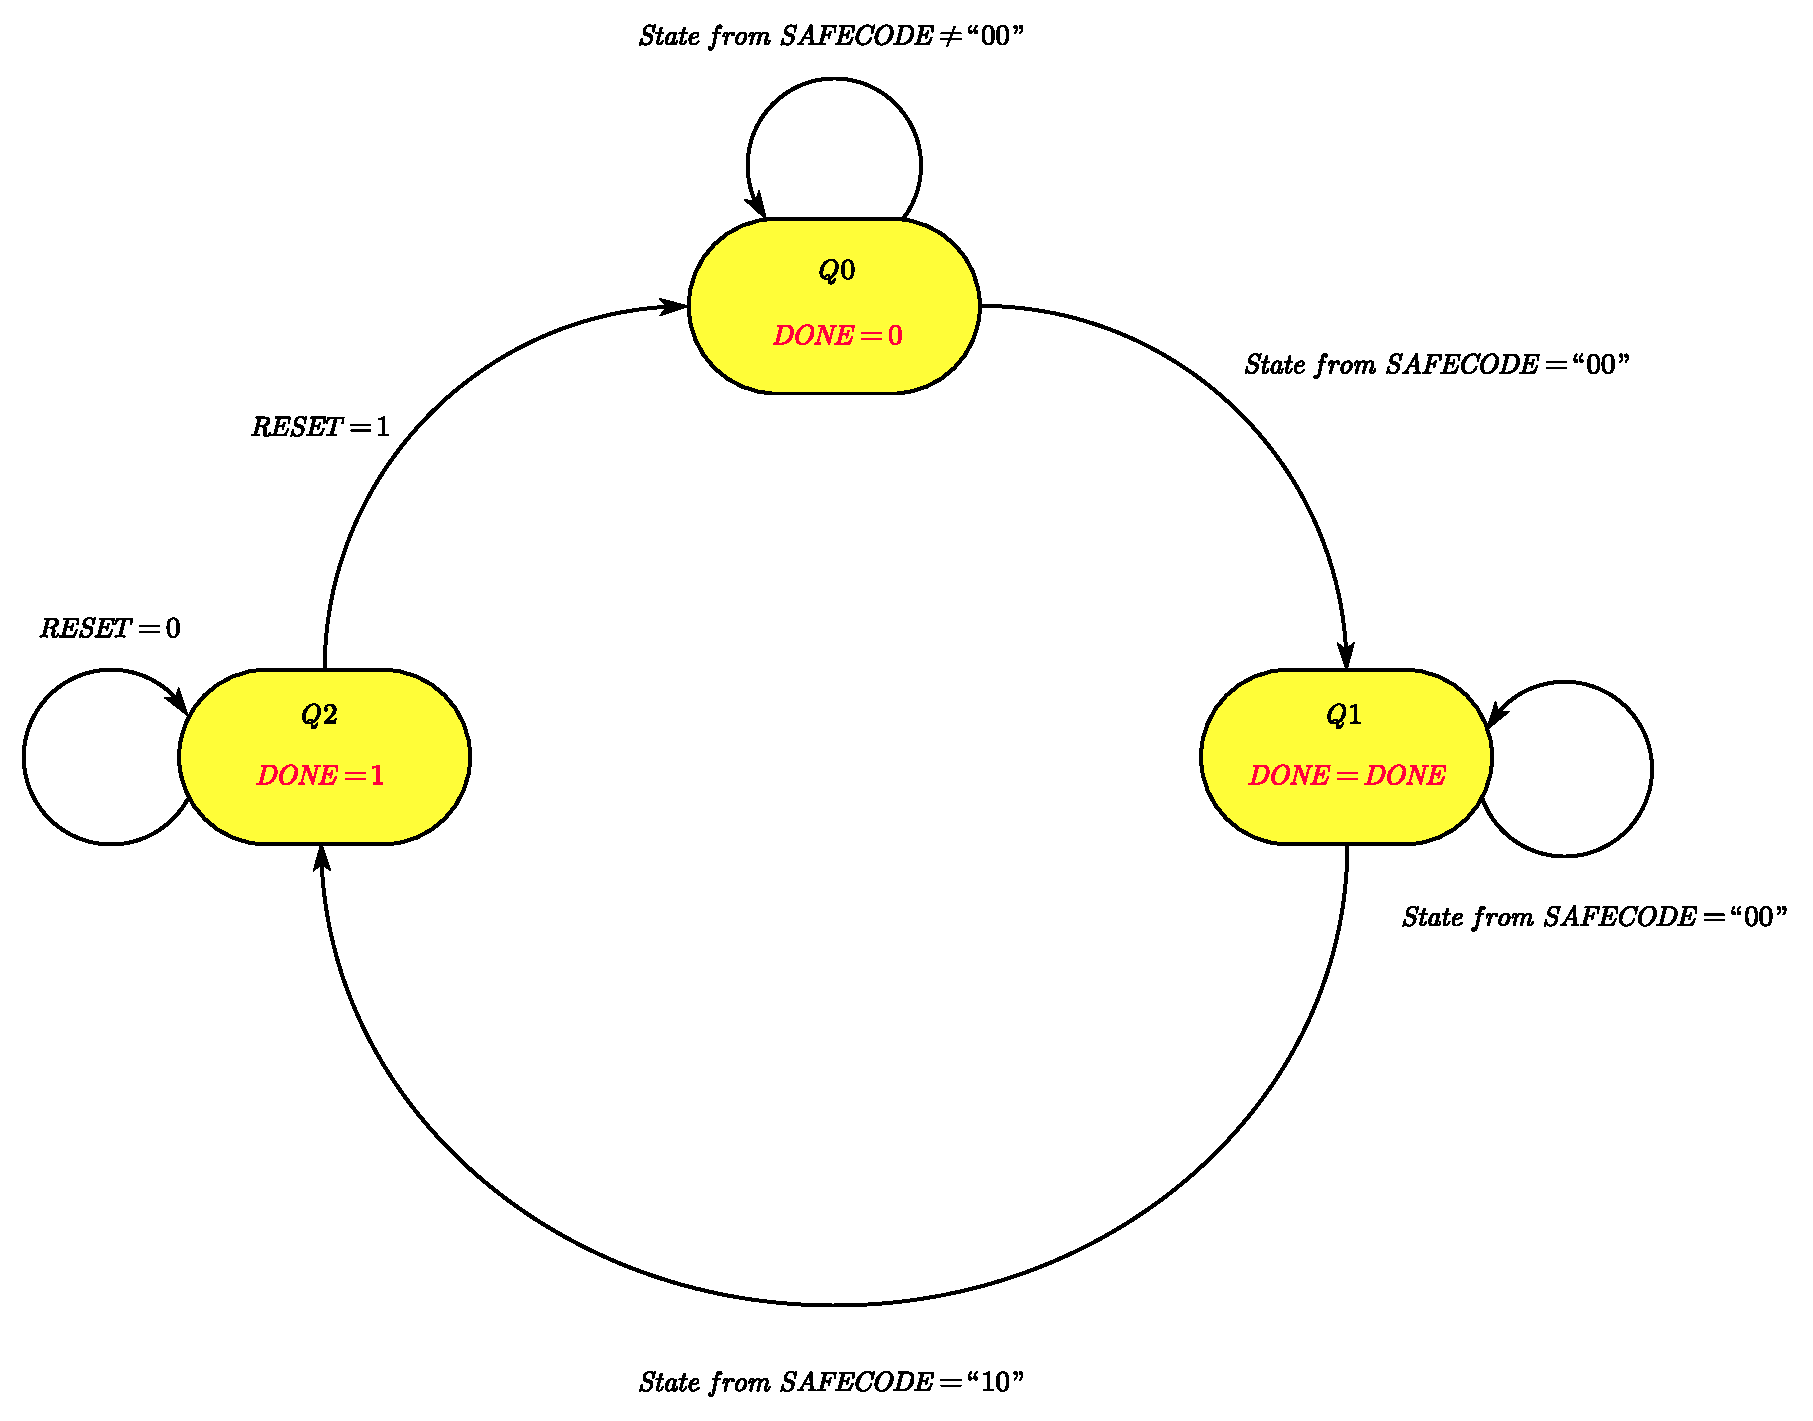
\includegraphics[scale = 0.49]{Graphics/STATE_FSM + DISPLAY/STATE_FSM.pdf}
    \caption{State\_FSM FSM}
    \label{fig:STATE_FSM_FSM}
\end{figure}

\vspace{0.6cm}

The VHDL code for this GAL can be found below: \bigskip

\inputcode{Code/STATE_FSM.vhd}


\clearpage

\subsubsection{Display}
\label{sec:DISPLAY}

DISPLAY has, as an input, the clock signal (\textit{CLK}) and \textit{DONE} signal from STATE\_FSM. Also, it has as outputs \textit{SEL}, a 4 bit signal which acts as a ring counter for the 4 digit 7 segment displays, \textit{A\_OUT}, a 2-bit vector that controls the addressing of the RAM,  \textit{WE\_OUT} and \textit{CS\_OUT}, being the Write Enable and Chip Select commanding signals for the RAM module.\medskip

Due to the fact that there is more than one GAL connected to the RAM to both read and write to it, as well as to the display, the use of tri-state buffers is necessary so as to avoid short circuits. The tri-state buffers act as switches commanded by CS\_OUT,  A\_OUT \& WE\_OUT. The output of these “switches” are the $\overline{CS}$, A \& $\overline{WE}$ signals needed to control the RAM IC.\medskip

We will now go over the different states that form this Finite State Machine:\bigskip

\textbf{Initialization Stage}\medskip

Every time that DONE is in LOW level, all the outputs are initialized at ‘0’. \medskip

\textbf{Ring (\textit{\bm{$Q_0$}, \bm{$Q_1$}, \bm{$Q_2$}, \bm{$Q_3$}})}
\medskip

Once DONE changes its value to HIGH,  WE\_OUT and CS\_OUT switch to HIGH level as well, enabling the tri-state buffers and pulling $\overline{WE} = 1$ and $\overline{CS}=0$ in order to put the RAM into Read Mode so as to show, at [D0...D3] the corresponding number depending on the address A\_OUT.\medskip

So, in the FSM of this GAL, in each of the states, A\_OUT will have a value for an address, at the same time, SEL will change the position of its HIGH level bit, turning one of the 4  7-segment display ON at a time, with the rest being OFF. Since the clock frequency is high, displaying only one number per clock frequency is enough to trick the human eye into believing that the 4 numbers are being displayed at the same time. This is done in such a way that the sequence of numbers that are being shown correspond to the ones stored in the RAM.\medskip

\medskip
{ \textbf{End of Ring}}
\medskip

If the ring passes through \textit{$Q_0$} and the DONE signal is in a LOW level, the ring stops and the system returns to the initialization stage.  


To show the numbers in the display, we have fashioned a custom 7-segment display driver. We can see it in the following image:

\begin{figure}[H]
    \centering
    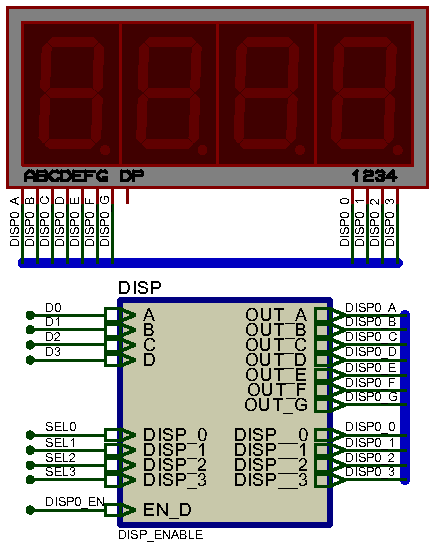
\includegraphics[scale = 0.9]{Graphics/STATE_FSM + DISPLAY/DISP_ENABLE.PDF}
    \caption{Proteus Subassembly of 7-segment display driver}
    \label{fig:DISP_ENABLE}
\end{figure}

The internals of this driver are composed of a 74247 display driver and some tri-state buffers to control when the driver is on, as well as to prevent short circuits in the outputs of the driver/inputs of the display. As we said before, this is due to the fact that the display is driven by different GALs, so we want a High-Z output in the drivers that are not in use. The \textit{EN\_D} signal is provided by another GAL that takes care of selecting which signal to display. (See \textbf{Subsubsection} \textbf{\ref{sec:ENABLE_SEL}} for more on this). We can see this internals here:

\begin{figure}[H]
    \centering
    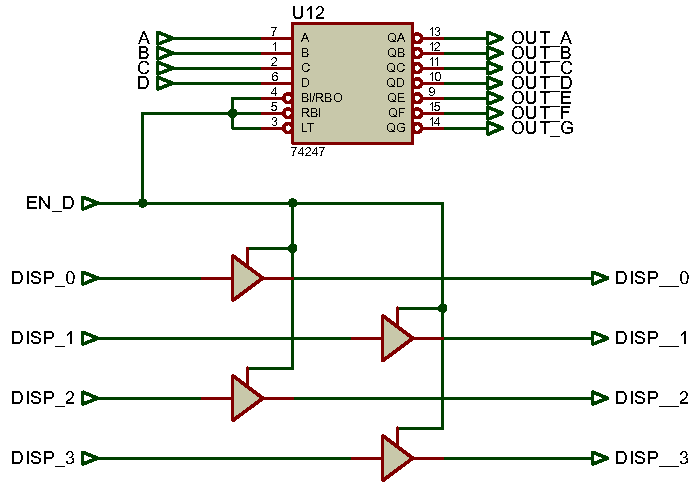
\includegraphics[scale = 0.8]{Graphics/STATE_FSM + DISPLAY/DISP_ENABLE_INT.PDF}
    \caption{7-segment display driver internals}
    \label{fig:DISP_ENABLE_INT}
\end{figure}

\clearpage

To illustrate the different states and the transitions between them we have included the following diagram:\medskip

\begin{figure}[H]
    \centering
    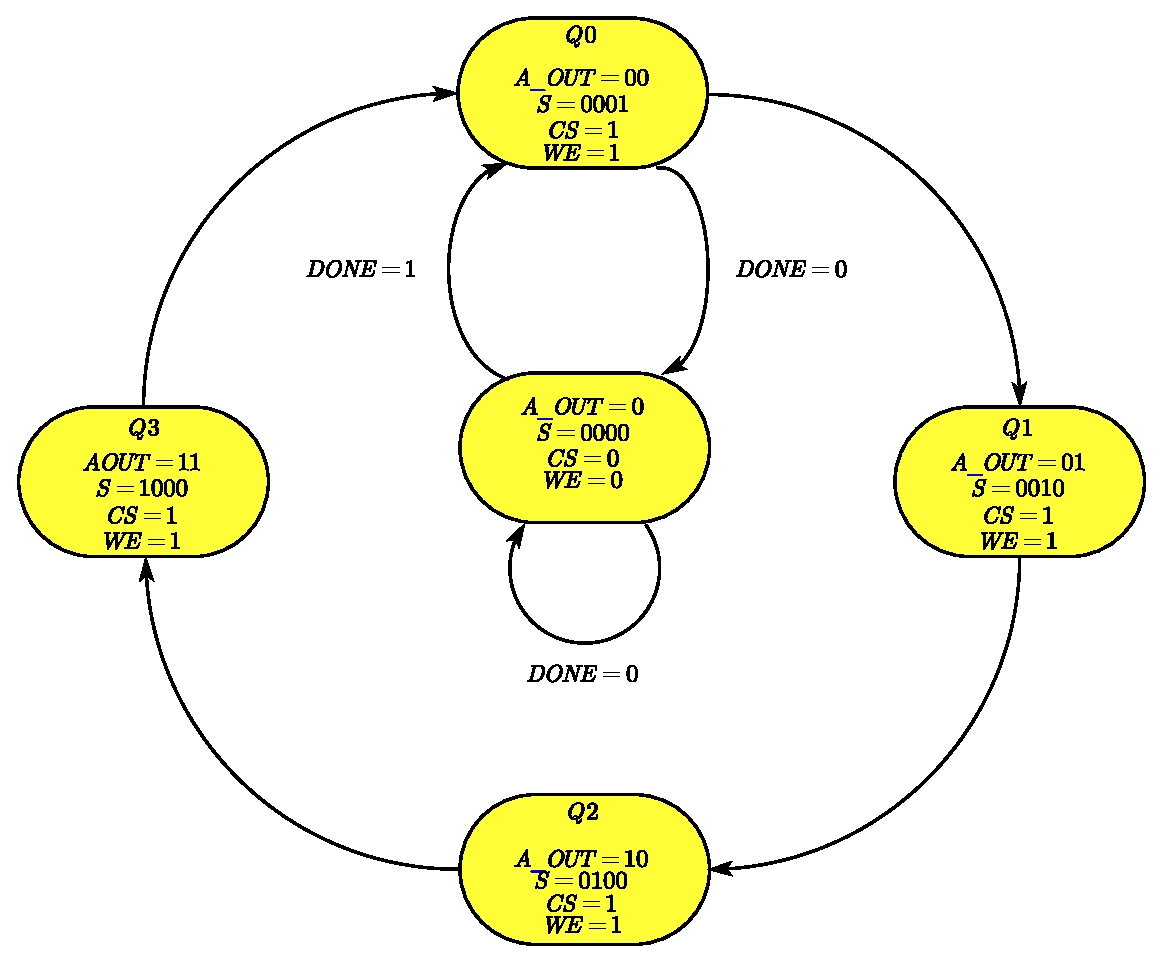
\includegraphics[scale = 0.55]{Graphics/STATE_FSM + DISPLAY/DISPLAY_FSM.pdf}
    \caption{Display FSM}
    \label{fig:DISPLAY_FSM_FSM}
\end{figure}

\vspace{0.5cm}

The final subassembly of both GALs can be seen here:

\begin{figure}[H]
    \centering
    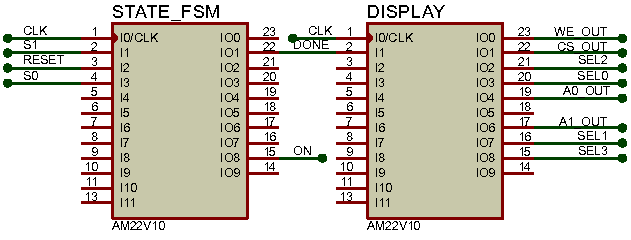
\includegraphics[scale = 1]{Graphics/STATE_FSM + DISPLAY/PROTEUS_BOTH.PDF}
    \caption{Proteus Subassembly of both GALs}
    \label{fig:PROTEUS_STATE_FSM_DISPLAY}
\end{figure}

\clearpage

The VHDL code is attached below:

\vspace{-0.1cm}

\inputcode{Code/DISPLAY.vhd}

\subsubsection{Final Roundup}
\label{sec:STATE_FSM_DISPLAY_ROUNDUP}

We know that this section may strike as a bit complex or hard to understand, so we will try to break down the different actions that both GALs perform in an step by step description of the procedure.

\begin{enumerate}
    \item The STATE\_FSM reads the state of SAFECODE using the state outputs of the latter.
    
    \item Once it detects a "00" it knows that the password is being entered.
    
    \item As soon as it reads a "10" (Last State of SAFECODE, triggered by the \textit{\#} key), it knows that all numbers have been entered and so it turns the \textit{DONE} pin ON.
    
    \item DISPLAY reads the \textit{DONE} pin and as soon as it turns ON, it starts a ring counter that sweeps through the 4 7-segment displays activating one each time. At the same time, the RAM is put into Read mode and the addresses are swept as well. In essence, the first displays turns on (with the rest off) and it displays the contents of Address = "00", then the second display turns on and displays Adress "01", and so on. This happens very fast, tricking the person into believing that all 4 displays are ON simultaneously.
    
    \item Once the \textit{RESET} signal is received by STATE\_FSM, the \textit{DONE} pin is pulled LOW and both GALs are reset.
\end{enumerate}



